\documentclass[border=4pt]{standalone}
\usepackage{tikz}
\usepackage{amsmath,amssymb}
\usepackage{mathptmx}
\usetikzlibrary{arrows.meta,positioning,calc,shapes.geometric,decorations.pathreplacing,shadows,fadings,patterns}
\definecolor{cblue}{HTML}{1F4E9C}
\definecolor{cgold}{HTML}{D08C00}
\definecolor{cred}{HTML}{B5172E}
\definecolor{cgreen}{HTML}{1B7A3A}
\definecolor{cgrey}{HTML}{555555}
\definecolor{cpurple}{HTML}{5B2A86}
% oblique 3D cuboid: \cuboid{x}{y}{z}{dx}{dy}{dz}{colour}
\newcommand{\cuboid}[7]{%
  \fill[#7!55!white,draw=#7!60!black,line width=0.4pt] (#1,#2,#3+#6) -- ++(#4,0,0) -- ++(0,#5,0) -- ++(-#4,0,0) -- cycle;
  \fill[#7!80!black,draw=#7!60!black,line width=0.4pt] (#1+#4,#2,#3) -- ++(0,#5,0) -- ++(0,0,#6) -- ++(0,-#5,0) -- cycle;
  \fill[#7,draw=#7!60!black,line width=0.4pt] (#1,#2,#3) -- ++(#4,0,0) -- ++(0,0,#6) -- ++(-#4,0,0) -- cycle;}

\begin{document}
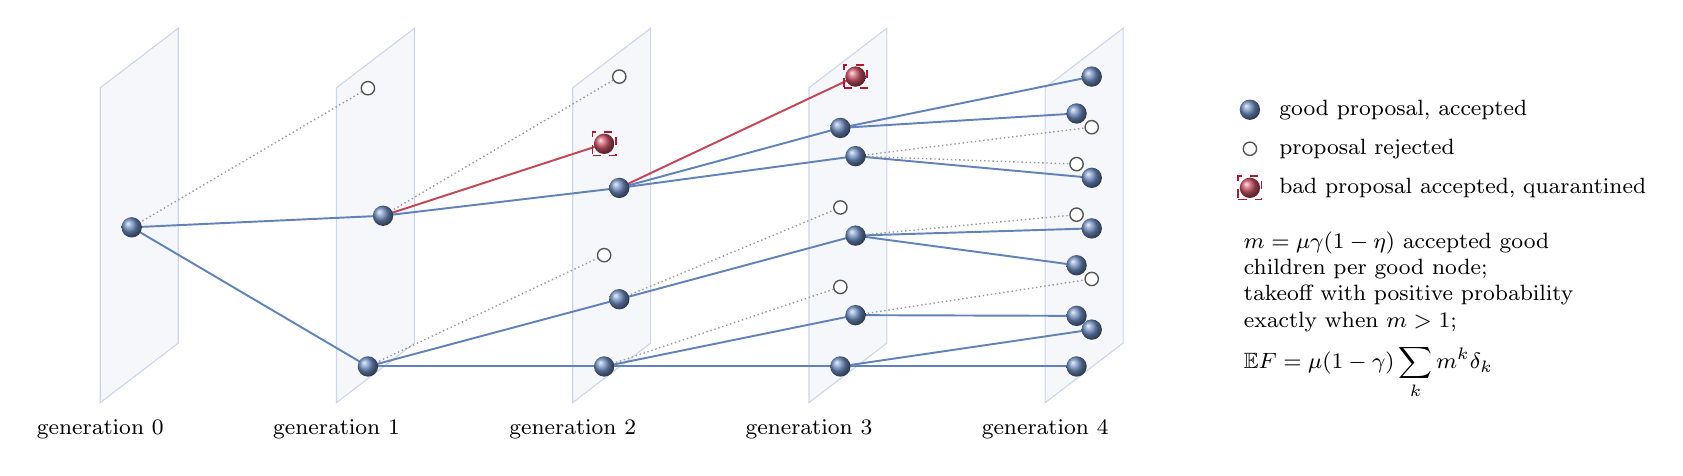
\begin{tikzpicture}[x={(1cm,0cm)},y={(0.55cm,0.42cm)},z={(0cm,0.62cm)},
  good/.style={circle,inner sep=2.6pt,ball color=cblue!65!white,draw=none},
  bad/.style={circle,inner sep=2.6pt,ball color=cred!75!white,draw=none},
  rej/.style={circle,inner sep=1.7pt,draw=cgrey,fill=white,line width=0.5pt},
  quar/.style={rectangle,inner sep=4.2pt,draw=cred,line width=0.6pt,dashed},
  edgeG/.style={cblue!70,line width=0.7pt},
  edgeR/.style={cgrey!60,line width=0.5pt,densely dotted},
  edgeB/.style={cred!80,line width=0.7pt}]
% generation sheets
\foreach \k in {0,...,4}{
  \pgfmathsetmacro\xx{3*\k}
  \fill[cblue!5,draw=cblue!25,line width=0.4pt,opacity=0.9] (\xx,0,0) -- (\xx,1.8,0) -- (\xx,1.8,6.45) -- (\xx,0,6.45) -- cycle;
  \node[font=\footnotesize,anchor=north] at (\xx,0,-0.15) {generation $\k$};}
\draw[edgeG] (0.000,0.725,3.100) -- (3.000,0.725,0.250);
\draw[edgeG] (0.000,0.725,3.100) -- (3.000,1.075,3.100);
\draw[edgeR] (0.000,0.725,3.100) -- (3.000,0.725,5.950);
\draw[edgeG] (3.000,0.725,0.250) -- (6.000,0.725,0.250);
\draw[edgeG] (3.000,0.725,0.250) -- (6.000,1.075,1.390);
\draw[edgeR] (3.000,0.725,0.250) -- (6.000,0.725,2.530);
\draw[edgeG] (3.000,1.075,3.100) -- (6.000,1.075,3.670);
\draw[edgeB] (3.000,1.075,3.100) -- (6.000,0.725,4.810);
\draw[edgeR] (3.000,1.075,3.100) -- (6.000,1.075,5.950);
\draw[edgeG] (6.000,0.725,0.250) -- (9.000,0.725,0.250);
\draw[edgeG] (6.000,0.725,0.250) -- (9.000,1.075,1.064);
\draw[edgeR] (6.000,0.725,0.250) -- (9.000,0.725,1.879);
\draw[edgeG] (6.000,1.075,1.390) -- (9.000,1.075,2.693);
\draw[edgeR] (6.000,1.075,1.390) -- (9.000,0.725,3.507);
\draw[edgeG] (6.000,1.075,3.670) -- (9.000,1.075,4.321);
\draw[edgeG] (6.000,1.075,3.670) -- (9.000,0.725,5.136);
\draw[edgeB] (6.000,1.075,3.670) -- (9.000,1.075,5.950);
\draw[edgeG] (9.000,0.725,0.250) -- (12.000,0.725,0.250);
\draw[edgeG] (9.000,0.725,0.250) -- (12.000,1.075,0.768);
\draw[edgeG] (9.000,1.075,1.064) -- (12.000,0.725,1.286);
\draw[edgeR] (9.000,1.075,1.064) -- (12.000,1.075,1.805);
\draw[edgeG] (9.000,1.075,2.693) -- (12.000,0.725,2.323);
\draw[edgeG] (9.000,1.075,2.693) -- (12.000,1.075,2.841);
\draw[edgeR] (9.000,1.075,2.693) -- (12.000,0.725,3.359);
\draw[edgeG] (9.000,1.075,4.321) -- (12.000,1.075,3.877);
\draw[edgeR] (9.000,1.075,4.321) -- (12.000,0.725,4.395);
\draw[edgeR] (9.000,1.075,4.321) -- (12.000,1.075,4.914);
\draw[edgeG] (9.000,0.725,5.136) -- (12.000,0.725,5.432);
\draw[edgeG] (9.000,0.725,5.136) -- (12.000,1.075,5.950);
\node[good] at (0.000,0.725,3.100) {};
\node[good] at (3.000,0.725,0.250) {};
\node[good] at (3.000,1.075,3.100) {};
\node[rej] at (3.000,0.725,5.950) {};
\node[good] at (6.000,0.725,0.250) {};
\node[good] at (6.000,1.075,1.390) {};
\node[rej] at (6.000,0.725,2.530) {};
\node[good] at (6.000,1.075,3.670) {};
\node[bad] at (6.000,0.725,4.810) {};
\node[quar] at (6.000,0.725,4.810) {};
\node[rej] at (6.000,1.075,5.950) {};
\node[good] at (9.000,0.725,0.250) {};
\node[good] at (9.000,1.075,1.064) {};
\node[rej] at (9.000,0.725,1.879) {};
\node[good] at (9.000,1.075,2.693) {};
\node[rej] at (9.000,0.725,3.507) {};
\node[good] at (9.000,1.075,4.321) {};
\node[good] at (9.000,0.725,5.136) {};
\node[bad] at (9.000,1.075,5.950) {};
\node[quar] at (9.000,1.075,5.950) {};
\node[good] at (12.000,0.725,0.250) {};
\node[good] at (12.000,1.075,0.768) {};
\node[good] at (12.000,0.725,1.286) {};
\node[rej] at (12.000,1.075,1.805) {};
\node[good] at (12.000,0.725,2.323) {};
\node[good] at (12.000,1.075,2.841) {};
\node[rej] at (12.000,0.725,3.359) {};
\node[good] at (12.000,1.075,3.877) {};
\node[rej] at (12.000,0.725,4.395) {};
\node[rej] at (12.000,1.075,4.914) {};
\node[good] at (12.000,0.725,5.432) {};
\node[good] at (12.000,1.075,5.950) {};

% legend
\begin{scope}[shift={(14.6,0,0)}]
\node[good] at (0,0,6.0) {}; \node[font=\footnotesize,anchor=west] at (0.25,0,6.0) {good proposal, accepted};
\node[rej] at (0,0,5.2) {}; \node[font=\footnotesize,anchor=west] at (0.25,0,5.2) {proposal rejected};
\node[bad] at (0,0,4.4) {}; \node[quar] at (0,0,4.4) {}; \node[font=\footnotesize,anchor=west] at (0.25,0,4.4) {bad proposal accepted, quarantined};
\node[font=\footnotesize,anchor=north west,align=left] at (-0.2,0,3.7) {$m=\mu\gamma(1-\eta)$ accepted good\\ children per good node;\\ takeoff with positive probability\\ exactly when $m>1$;\\[4pt]
 $\mathbb{E}F=\mu(1-\gamma)\displaystyle\sum_k m^k\delta_k$};
\end{scope}
\end{tikzpicture}
\end{document}
